

%% AAPT Physics Bowl Exams Questions
%%----------------------------------------


%% This section has XX problems


%% PhysicsBowl 2015
%%----------------------------------------
\element{aapt}{ %% Bowl-B2
\begin{question}{bowl-2015-q34}
    An upward-pointing object is placed \SI{15.0}{\centi\meter} to the left of a lens system.
    The first lens is convex with focal length \SI{10.0}{\centi\meter}.
    The second lens is convex with focal length \SI{10}{\centi\meter} and its location from the first lens is varied from \SI{10}{\centi\meter} away to \SI{110}{\centi\meter} away.
    \emph{Please Note:} not drawn to scale.
    \begin{center}
    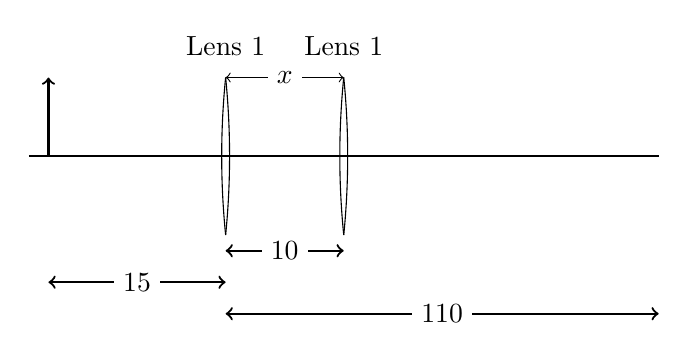
\begin{tikzpicture}
        %% optical axis
        \draw[thick] (-3,0) -- (5,0);
        %% object
        \draw[thick,->] (-2.75,0) -- (-2.75,1);
        %% lens 1
        \draw (-0.5,1) arc (5.74:-5.74:10);
        \draw (-0.5,1) arc (174.26:185.74:10);
        \node[anchor=south,yshift=1ex] at (-0.5,1) {Lens 1};
        %% lens 2
        \draw (+1,1) arc (5.74:-5.74:10);
        \draw (+1,1) arc (174.26:185.74:10);
        \node[anchor=south,yshift=1ex] at (+1,1) {Lens 1};
        %% distance x
        \draw[<->] (-0.5,1) -- (+1,1) node[pos=0.5,anchor=center,fill=white] {$x$};
        \draw[thick,<->] (-0.5,-1.2) -- (+1,-1.2) node[pos=0.5,anchor=center,fill=white] {\SI{10}{\centi\meter}};
        \draw[thick,<->] (-0.5,-1.6) -- (-2.75,-1.6) node[pos=0.5,anchor=center,fill=white] {\SI{15}{\centi\meter}};
        \draw[thick,<->] (-0.5,-2) -- (+5,-2) node[pos=0.5,anchor=center,fill=white] {\SI{110}{\centi\meter}};
    \end{tikzpicture}
    \end{center}
    Which one of the following choices best represents the description of the final image formed as the second lens is moved from $x=\SI{10}{\centi\meter}$ to $x=\SI{110}{\centi\meter}$ from the first lens?
    \begin{center}
    \begin{tabu}{cX[c]X[c]X[c]}
        \toprule
        \makebox[1.5em][c]{\textnumero}
            & $x=\SI{10}{\centi\meter}$
            & $\longrightarrow~~~\longrightarrow~~~\longrightarrow$
            & $x=\SI{110}{\centi\meter}$ \\
        \bottomrule
    \end{tabu}
    \end{center}
    \begin{choices}
        \correctchoice{
            \begin{tabu}{X[c]X[c]X[c]}
                Real and pointing downward & Virtual and pointing downward & Real and pointing upward \\
                \midrule
            \end{tabu}
        }
        \wrongchoice{
            \begin{tabu}{X[c]X[c]X[c]}
                Virtual and pointing downward & Virtual and pointing upward & Real and pointing upward \\
                \midrule
            \end{tabu}
        }
        \wrongchoice{
            \begin{tabu}{X[c]X[c]X[c]}
                Virtual and pointing upward & Virtual and pointing downward & Real and pointing upward \\
                \midrule
            \end{tabu}
        }
        \wrongchoice{
            \begin{tabu}{X[c]X[c]X[c]}
                Real and pointing upward & Virtual and pointing downward & Real and pointing upward \\
                \midrule
            \end{tabu}
        }
        \wrongchoice{
            \begin{tabu}{X[2c]X[c]}
                Virtual and pointing downward & Real and pointing upward \\
                \midrule
            \end{tabu}
        }
    \end{choices}
\end{question}
}

\element{aapt}{ %% Bowl-B2
\begin{question}{bowl-2015-q38}
    A thin film of alcohol ($n_{alcohol}=1.35$) lies on a flat glass surface ($n_{glass}=1.60$).
    When light of wavelength \SI{540}{\nano\meter} is incident normal to the alcohol surface from air,
        the light is strongly reflected, but when light of wavelength \SI{432}{\nano\meter}
        is incident normal to the surface from air, the reflected light is minimized.
    \begin{center}
    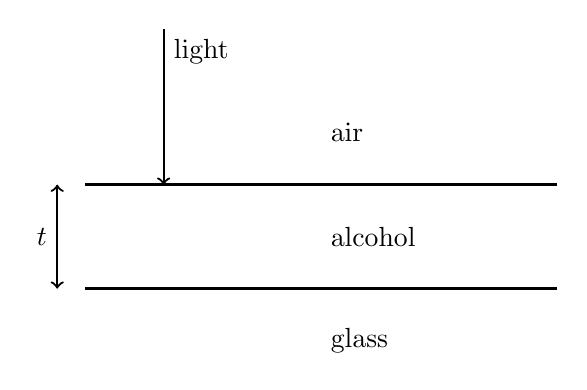
\begin{tikzpicture}[yscale=0.66]
        %% Boundaries
        \draw[very thick] (0,2) -- (6,2);
        \draw[very thick] (0,0) -- (6,0);
        %% Lebels
        \node[anchor=west] at (3,3) {air};
        \node[anchor=west] at (3,1) {alcohol};
        \node[anchor=west] at (3,-1) {glass};
        %% Thickness
        \draw[thick,<->] (-1em,0) -- (-1em,2) node[pos=0.5,anchor=east] {$t$};
        %% Incoming Ray
        \draw[thick,->] (1,5) -- (1,2) node[pos=0.0,anchor=north west] {light};
    \end{tikzpicture}
    \end{center}
    Which one of the following choices could represent the thickness, $t$, of the alcohol film?
    \begin{multicols}{3}
    \begin{choices}
        \wrongchoice{\SI{216}{\nano\meter}}
        \wrongchoice{\SI{320}{\nano\meter}}
        \wrongchoice{\SI{324}{\nano\meter}}
      \correctchoice{\SI{400}{\nano\meter}}
        \wrongchoice{\SI{486}{\nano\meter}}
    \end{choices}
    \end{multicols}
\end{question}
}


%% PhysicsBowl 2014
%%----------------------------------------
\element{aapt}{ %% Bowl-B2
\begin{question}{bowl-2014-q25}
    It is observed that a light ray changes direction when it enters a new material.
    Which one of the following choices is the term best associated with this phenomenon?
    \begin{multicols}{2}
    \begin{choices}
        \wrongchoice{Doppler Effect}
        \wrongchoice{Interference}
        \wrongchoice{Polarization}
        \wrongchoice{Diffraction}
      \correctchoice{Refraction}
    \end{choices}
    \end{multicols}
\end{question}
}

\element{aapt}{ %% Bowl-B2
\begin{question}{bowl-2014-q36}
    A concave mirror with focal length $f$ is shown in the figure.
    \begin{center}
    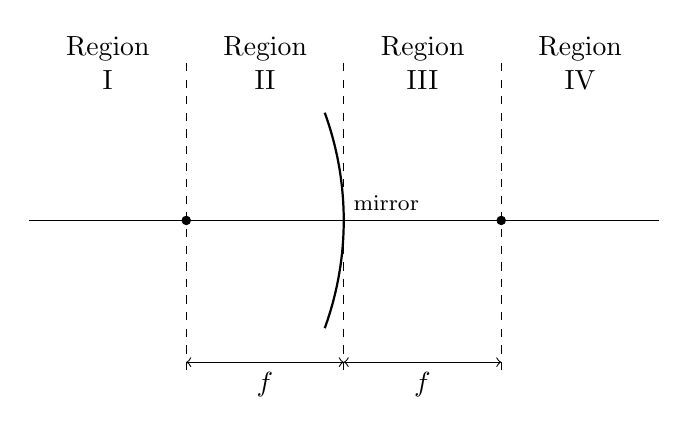
\begin{tikzpicture}
        %% Optical axis
        \draw (-4,0) -- (4,0);
        \draw[fill] (-2,0) circle (1.5pt);
        \draw[fill] (+2,0) circle (1.5pt);
        %% Region Labels
        \node[anchor=center,text width=3em,text centered] at (-3,2) {Region I};
        \node[anchor=center,text width=3em,text centered] at (-1,2) {Region II};
        \node[anchor=center,text width=3em,text centered] at (+1,2) {Region III};
        \node[anchor=center,text width=3em,text centered] at (+3,2) {Region IV};
        %% Region lines
        \draw[dashed] (2,2) -- (2,-2);
        \draw[dashed] (0,2) -- (0,-2);
        \draw[dashed] (-2,2) -- (-2,-2);
        %% Mirror
        \draw[thick] (-4,0) ++ (-20:4) arc (-20:20:4);
        \node[font=\footnotesize,anchor=south west] at (0,0) {mirror};
        %% Focal Lengths
        \draw[<->] (-2,-1.8) -- (0,-1.8) node[pos=0.5,anchor=north] {$f$};
        \draw[<->] (+2,-1.8) -- (0,-1.8) node[pos=0.5,anchor=north] {$f$};
    \end{tikzpicture}
    \end{center}
    A real object now is placed to the left of the mirror.
    In theory, which one of the following choices best describes everywhere that it is impossible for an image to form from the mirror?
    \begin{choices}
      \correctchoice{Region II only.}
        \wrongchoice{Region II and III only.}
        \wrongchoice{Region III and IV only.}
        \wrongchoice{Region II and IV only.}
        \wrongchoice{Region I, II, and IV only.}
    \end{choices}
\end{question}
}

\element{aapt}{ %% Bowl-B2
\begin{question}{bowl-2014-q44}
    A ray of monochromatic light enters the right-triangular glass as shown.
    \begin{center}
    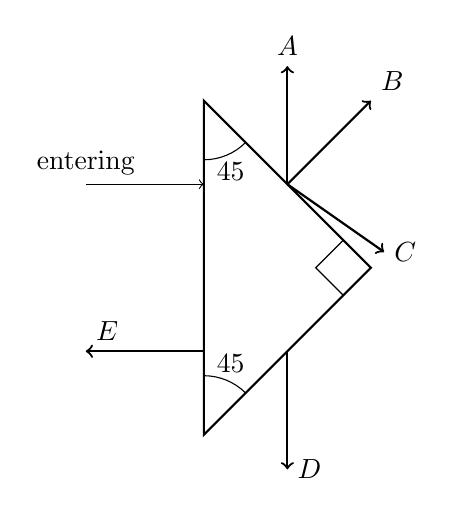
\begin{tikzpicture}[scale=0.75]
        %% Define corners of prism
        \coordinate (A) at (0,0);
        \coordinate (B) at (0,5.656);
        \coordinate (C) at (2.828,2.828);
        \draw[thick] (A) -- (B) -- (C) -- cycle;
        %% Angle labels
        \draw (A) ++ (45:1.00) arc (45:90:1.00) node[pos=0.4,anchor=south] {\ang{45}};
        \draw (B) ++ (270:1.00) arc (270:315:1.00) node[pos=0.6,anchor=north] {\ang{45}};
        \draw (C) ++ (225:0.66) -- ++ (135:0.66) -- ++ (45:0.66);
        %% Entering
        \draw[<-] (B) ++ (270:1.414cm) -- ++ (180:2cm) node[pos=1.0,anchor=south] {entering};
        %% Options
        \draw[thick,->] (B) ++ (-45:2cm) -- ++ (90:2cm) node[pos=1.0,anchor=south] {$A$};
        \draw[thick,->] (B) ++ (-45:2cm) -- ++ (45:2cm) node[pos=1.0,anchor=south west] {$B$};
        \draw[thick,->] (B) ++ (-45:2cm) -- ++ (-35:2cm) node[pos=1.0,anchor=west] {$C$};
        \draw[thick,->] (A) ++ (45:2cm) -- ++ (270:2cm) node[pos=1.0,anchor=west] {$D$};
        \draw[thick,->] (A) ++ (90:1.414cm) -- ++ (180:2cm) node[pos=1.0,anchor=south west] {$E$};
    \end{tikzpicture}
    \end{center}
    %% NOTE: critical angle for crown glass is 41 = asin( 1/1.52 )
    Which one of the lettered rays shows the path of the light after it exits the glass?
    \begin{multicols}{5}
    \begin{choices}[o]
        \wrongchoice{$A$}
        \wrongchoice{$B$}
        \wrongchoice{$C$}
        \wrongchoice{$D$}
      \correctchoice{$E$}
    \end{choices}
    \end{multicols}
\end{question}
}


%% PhysicsBowl 2013
%%----------------------------------------
\element{aapt}{ %% Bowl-B2
\begin{question}{bowl-2013-q27}
    Light of wavelength \SI{600}{\nano\meter} is transmitted from air into a piece of glass.
    \begin{center}
    \begin{tikzpicture}
    \begin{scope}[decoration={markings,mark=at position 0.5 with {\arrow{latex}}}] 
        %% 30, 60 triangle
        \draw[thick] (0,0) -- (-6.93,0) -- (-6.93,4) -- cycle;
        \node[anchor=south west,shift={(1ex,1ex)}] at (-6.93,0) {Glass};
        %% incoming
        \draw[thick,postaction={decorate}] (0,2) -- (-3.46,2);
        %% refracted
        \foreach \x/\y in {160/A,180/B,206/C}
            \draw[thick,postaction={decorate}] (-3.46,2) -- ++ (\x:1.73) node[anchor=center,shift={(\x:1em)}] {$\y$};
        \foreach \x/\y in {270/D,290/E}
            \draw[thick,postaction={decorate}] (-3.46,2) -- ++ (\x:1.41) node[anchor=center,shift={(\x:1em)}] {$\y$};
    \end{scope}
    \end{tikzpicture}
    \end{center}
    Which one of the labeled arrows best indicates the path of the light ray after it enters the glass?
    \begin{multicols}{5}
    \begin{choices}[o]
        \wrongchoice{$A$}
        \wrongchoice{$B$}
      \correctchoice{$C$}
        \wrongchoice{$D$}
        \wrongchoice{$E$}
    \end{choices}
    \end{multicols}
\end{question}
}

\element{aapt}{ %% Bowl-B2
\begin{question}{bowl-2013-q37}
    A real object in air is placed in front of a glass lens.
    The calculated image size is larger than the size of the original object.
    Which one of the following conclusions about the type of lens used and the type of image formed is correct?
    \begin{center}
    \begin{tabu}{cX[2c]X[3c]}
        \toprule
        \makebox[1.5em][c]{\textnumero}
            & Type of Lens & Type of Image \\
        \bottomrule
    \end{tabu}
    \end{center}
    \begin{choices}
      \correctchoice{\begin{tabu}{X[2c]X[3c]} Convex only & Could be virtual or real \\ \end{tabu}}
        \wrongchoice{\begin{tabu}{X[2c]X[3c]} Concave only & Will be virtual only \\ \end{tabu}}
        \wrongchoice{\begin{tabu}{X[2c]X[3c]} Either concave or convex & Will be virtual only \\ \end{tabu}}
        \wrongchoice{\begin{tabu}{X[2c]X[3c]} Convex only & Will be real only \\ \end{tabu}}
        \wrongchoice{\begin{tabu}{X[2c]X[3c]} Either concave or convex & Virtual for the concave lens; Real for the convex lens \\ \end{tabu}}
    \end{choices}
\end{question}
}


%% PhysicsBowl 2012
%%----------------------------------------
\element{aapt}{ %% Bowl-B2
\begin{question}{bowl-2012-q02}
    A ray of light passes straight downward through the point labeled $B$ in the diagram shown.
    The ray reaches a flat mirror placed at an angle $\theta$ to the horizontal as shown.
    \begin{center}
    \begin{tikzpicture}
        %% mirror
        \draw[very thick] (0,0) -- (150:6) node[pos=0.75,anchor=north,rotate=-30] {mirror};
        %% horizontal
        \draw[dashed] (0,0) -- (-5,0);
        \draw[<->] (-1,0) arc(180:150:1) node[pos=0.5,anchor=east] {$\theta$};
        %% ray
        \draw[thick,<-] (60:2) ++(150:4) ++(90:1ex) -- ++(90:2) node[anchor=north west] {ray};
        %% options
        \foreach \x/\y in {0/D,2/C,4/B,6/A}
            \fill (60:2) ++ (150:\x) circle (2pt) node[anchor=south west] {$\y$};
        \fill ({-4*cos(30) + 2*sin(30)},1em) circle (2pt) node[anchor=east] {$E$};
    \end{tikzpicture}
    \end{center}
    Which one of the locations labeled in the figure best represents the point through which the ray reflected from the mirror will pass?
    \begin{multicols}{5}
    \begin{choices}[o]
        \wrongchoice{$A$}
        \wrongchoice{$B$}
      \correctchoice{$C$}
        \wrongchoice{$D$}
        \wrongchoice{$E$}
    \end{choices}
    \end{multicols}
\end{question}
}

\element{aapt}{ %% Bowl-B2
\begin{question}{bowl-2012-q35}
    A student wants to set up an experiment with a thin convex lens of focal length $f$ such that a thin real object produces a focused real image on a movable screen.
    At how many locations along the optical axis (principal axis) can the object be placed so that the distance between the object and the focused image on the screen is equal to $3f$?
    \begin{choices}
      \correctchoice{There is no location.}
        \wrongchoice{There is exactly one location.}
        \wrongchoice{There are exactly two locations.}
        \wrongchoice{There are exactly two locations.}
        \wrongchoice{There are an infinite number of locations.}
    \end{choices}
\end{question}
}


%% PhysicsBowl 2011
%%----------------------------------------
\element{aapt}{ %% Bowl-B2
\begin{question}{bowl-2011-q33}
    For the setup-up shown of a candle and screen placed \SI{30}{\centi\meter} apart,
        there are two locations at which a thin converging lens can be placed to produce a focused real image.
    \begin{center}
    \begin{tikzpicture}
        %% optical axis
        \draw (-1,0) -- (6.5,0);
        %% object (candle)
        \draw[thick,->] (0,0) -- (0,1) node[anchor=south] {candle};
        %% screen
        \draw[thick] (6,0) -- (6,2) node[anchor=south] {screen};
        \node[anchor=west,pattern=north east lines,minimum height=2cm] at (6,1) {};
        %% distance
        \draw[thick,<->] (0,-1em) -- (6,-1em) node[pos=0.5,anchor=center,fill=white] {\SI{30}{\centi\meter}};
    \end{tikzpicture}
    \end{center}
    One real image of the candle appears on the screen when the lens is located \SI{12}{\centi\meter} from the candle.
    From this location,
        how does this lens now have to moved in order to make the second real image of the candle appear on the screen?
    \begin{choices}
        \wrongchoice{\SI{3}{\centi\meter} toward the screen}
        \wrongchoice{\SI{6}{\centi\meter} toward the candle}
      \correctchoice{\SI{6}{\centi\meter} toward the screen}
        \wrongchoice{\SI{9}{\centi\meter} toward the candle}
        \wrongchoice{\SI{9}{\centi\meter} toward the screen}
    \end{choices}
\end{question}
}

\element{aapt}{ %% Bowl-B2
\begin{question}{bowl-2011-q45}
    An object is placed in front of a thin converging lens resulting in a focused image forming on a screen.
    If the bottom half of the lens were covered with black paper,
        what happens to the image on the screen?
    \begin{choices}
        \wrongchoice{There is no change of any kind to the image.}
        \wrongchoice{Only the top half of the image is focused into an image on the screen.}
        \wrongchoice{Only the top half of the object is focused into an image on the screen and it now is half the size.}
        \wrongchoice{The image is fully formed, only it is now half as large.}
      \correctchoice{The image is fully formed, only it is dimmer.}
    \end{choices}
\end{question}
}

\element{aapt}{ %% Bowl-B2
\begin{question}{bowl-2010-q28}
    Which of the following \emph{could} produce an enlarged but inverted image of a real object?
    \begin{choices}
      \correctchoice{Place a converging lens at a distance greater than its focal length from the object.}
        \wrongchoice{Place a converging lens at a distance less than its focal length from the object.}
        \wrongchoice{Place a diverging lens at a distance less than the magnitude of its focal length from the object.}
        \wrongchoice{Place a diverging lens at a distance greater than the magnitude of its focal length from the object.}
        \wrongchoice{It is not possible to create the type of image desired.}
    \end{choices}
\end{question}
}

\element{aapt}{ %% Bowl-B2
\begin{question}{bowl-2010-q30}
    Chromatic aberration from a lens is a consequence of:
    \begin{choices}
        \wrongchoice{polarization}
        \wrongchoice{interference}
        \wrongchoice{total internal reflection}
        \wrongchoice{diffraction}
      \correctchoice{dispersion}
    \end{choices}
\end{question}
}


%% PhysicsBowl 2008
%%----------------------------------------
\element{aapt}{ %% Bowl-B2
\begin{question}{bowl-2008-q21}
    Modern telescopes use mirrors, rather than lenses, to form images.
    One advantage of mirrors over lenses is that the images formed by mirrors are not affected by:
    \begin{choices}
        \wrongchoice{destructive interference}
        \wrongchoice{constructive interference}
      \correctchoice{chromatic aberration}
        \wrongchoice{spherical aberration}
        \wrongchoice{atmospheric refraction}
    \end{choices}
\end{question}
}

\element{aapt}{ %% Bowl-B2
\begin{question}{bowl-2008-q28}
    A diverging lens produces an image of a real object.
    The image is:
    \begin{choices}
        \wrongchoice{virtual, larger than the object, and upright.}
      \correctchoice{virtual, smaller than the object, and upright.}
        \wrongchoice{virtual, smaller than the object, and inverted.}
        \wrongchoice{real, smaller than the object, and inverted.}
        \wrongchoice{real, larger than the object, and inverted.}
    \end{choices}
\end{question}
}


%% PhysicsBowl 2006
%%----------------------------------------
\element{aapt}{ %% Bowl-B2
\begin{question}{bowl-2006-q38}
    For which of the following does one obtain an image of increased size from a real object?
    Take all focus and radius of curvature values as positive.
    \begin{choices}
        \wrongchoice{The object is placed at a position outside the radius of curvature for a converging lens.}
        \wrongchoice{The object is placed at a position outside the radius of curvature for a diverging lens.}
        \wrongchoice{The object is placed at a position inside the magnitude of the focus for a concave lens.}
      \correctchoice{The object is placed at a position between the focus and radius of curvature for a concave mirror.}
        \wrongchoice{The object is placed at a position between the focus and the radius of curvature for a convex mirror.}
    \end{choices}
\end{question}
}


%% PhysicsBowl 2005
%%----------------------------------------
\element{aapt}{ %% Bowl-B2
\begin{question}{bowl-2005-q18}
    A student holds a hand mirror to observe the back of her head while standing in front of and looking into a wall mirror.
    If she is standing \SI{4}{\foot} in front of the wall mirror and she holds the hand mirror \SI{1}{\foot} behind her head,
        she will see the back of her head how far behind the wall mirror?
    \begin{multicols}{3}
    \begin{choices}
      \correctchoice{\SI{6}{\foot}}
        \wrongchoice{\SI{5}{\foot}}
        \wrongchoice{\SI{4}{\foot}}
        \wrongchoice{\SI{3}{\foot}}
        \wrongchoice{\SI{2}{\foot}}
    \end{choices}
    \end{multicols}
\end{question}
}

\element{aapt}{ %% Bowl-B2
\begin{question}{bowl-2005-q26}
    Light shines from air into a clear material.
    When the light makes an angle of incidence equal to \ang{30.0},
        the light refracts at an angle of \ang{15.0}.
    If the light is shone from an angle of incidence of \ang{60.0},
        what is the angle of refraction?
    \begin{multicols}{3}
    \begin{choices}
        \wrongchoice{\ang{19.5}}
      \correctchoice{\ang{26.6}}
        \wrongchoice{\ang{30.0}}
        \wrongchoice{\ang{45.0}}
        \wrongchoice{\ang{60.0}}
    \end{choices}
    \end{multicols}
\end{question}
}

\element{aapt}{ %% Bowl-B2
\begin{question}{bowl-2005-q29}
    An object is in front of a convex lens,
        at a distance less than the focal length from the lens.
    Its image is:
    \begin{choices}
      \correctchoice{virtual and larger than the object.}
        \wrongchoice{real and smaller than the object.}
        \wrongchoice{virtual and smaller than the object.}
        \wrongchoice{real and larger than the object.}
        \wrongchoice{virtual and the same size as the object.}
    \end{choices}
\end{question}
}


%% PhysicsBowl 2000
%%----------------------------------------
\element{aapt}{ %% Bowl-B2
\begin{question}{bowl-2000-q01}
    As a wave moves from one medium to a second medium with a different index of refraction,
        which of the following wave properties would \emph{never} change?
    \begin{multicols}{2}
    \begin{choices}
      \correctchoice{frequency}
        \wrongchoice{wavelength}
        \wrongchoice{speed}
        \wrongchoice{angle}
        \wrongchoice{all will change}
    \end{choices}
    \end{multicols}
\end{question}
}

\element{aapt}{ %% Bowl-B2
\begin{question}{bowl-2000-q04}
    Specular reflection occurs whenever light is incident on:
    \begin{choices}
      \correctchoice{a smooth surface}
        \wrongchoice{a rough surface}
        \wrongchoice{a boundary between high index of refraction and low index of refraction materials}
        \wrongchoice{a boundary between low index of refraction and high index of refraction materials}
        \wrongchoice{a boundary between any two transparent substances, regardless of index of refraction}
    \end{choices}
\end{question}
}

\element{aapt}{ %% Bowl-B2
\begin{questionmult}{bowl-2000-q16}
    Consider an illuminated object, a pinhole,
        and a screen arranged to form a pinhole image on the screen.
    Which of the following will occur if the screen is moved away from the pinhole?
    \begin{choices}
        \wrongchoice{the image will go out of focus}
      \correctchoice{the image will become larger}
        \wrongchoice{the image will become brighter}
    \end{choices}
\end{questionmult}
}


%% PhysicsBowl 1999
%%----------------------------------------
\element{aapt}{ %% Bowl-B2
\begin{question}{bowl-1999-q34}
    A small light bulb is placed \SI{20}{\centi\meter} to the right of a converging lens of focal length \SI{10}{\centi\meter}.
    Which of the following statements is \emph{not} true about the image of the bulb formed by the lens?
    \begin{choices}
      \correctchoice{It is virtual.}
        \wrongchoice{It is inverted.}
        \wrongchoice{It is the same size as the bulb.}
        \wrongchoice{It is \SI{20}{\centi\meter} to the left of the lens.}
        \wrongchoice{It is can be projected on a screen.}
    \end{choices}
\end{question}
}

\element{aapt}{ %% Bowl-B2
\begin{question}{bowl-1999-q38}
    An image is formed on a screen by a convergent lens.
    If the top half of the lens is then covered what will happen to the image?
    \begin{choices}
      \correctchoice{the image is dimmer but otherwise unchanged.}
        \wrongchoice{the image becomes half as big.}
        \wrongchoice{only the top half of the image is produced.}
        \wrongchoice{only the bottom half of the image is produced.}
        \wrongchoice{the image becomes half as big and is inverted from its original position.}
    \end{choices}
\end{question}
}


%% PhysicsBowl 1998
%%----------------------------------------
\element{aapt}{ %% Bowl-B2
\begin{question}{bowl-1998-q04}
    As sound travels from steel into air,
        both its speed and its:
    \begin{choices}
        \wrongchoice{wavelength increase}
      \correctchoice{wavelength decrease}
        \wrongchoice{frequency increase}
        \wrongchoice{frequency decrease}
        \wrongchoice{frequency remain unchanged}
    \end{choices}
\end{question}
}

\element{aapt}{ %% bowl-B2
\begin{question}{bowl-1998-q19}
    In order to produce an enlarged, upright image of an object,
        you could use a:
    \begin{choices}
        \wrongchoice{converging lens more than one focal length from the object.}
      \correctchoice{converging lens less than one focal length from the object.}
        \wrongchoice{diverging lens more than one focal length from the object.}
        \wrongchoice{diverging lens exactly one focal length from the object.}
        \wrongchoice{diverging lens less than one focal length from the object.}
    \end{choices}
\end{question}
}

\element{aapt}{ %% Bowl-B2
\begin{question}{bowl-1998-q36}
    The critical angle in a transparent substance surrounded by air is \ang{30}.
    The speed of light in the substance (in multiples of \SI{e8}{\meter\per\second}) is most nearly:
    \begin{multicols}{3}
    \begin{choices}
        \wrongchoice{\num{1.0}}
      \correctchoice{\num{1.5}}
        \wrongchoice{\num{2.0}}
        \wrongchoice{\num{3.0}}
        \wrongchoice{\num{6.0}}
    \end{choices}
    \end{multicols}
\end{question}
}


%% PhysicsBowl 1997
%%----------------------------------------
\element{aapt}{ %% Bowl-B2
\begin{question}{bowl-1997-q07}
    A narrow beam of monochromatic light enters a lens parallel to the optic axis,
        as shown in the accompanying diagram.
    \begin{center}
    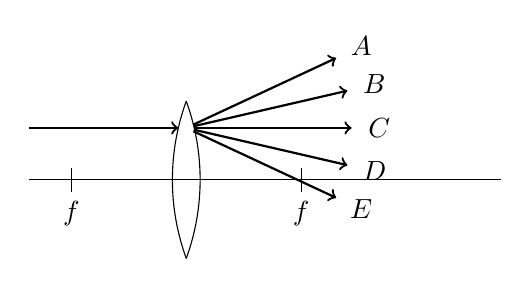
\begin{tikzpicture}
        %% optical axis
        \draw (-2,0) -- (4,0);
        %% lens
        \draw (0,1) arc (20:-20:2.92);
        \draw (0,1) arc (160:200:2.92);
        %% incoming
        \draw[thick,->] (-2,0.66) -- (-0.1,0.66);
        %% outgoing
        \foreach \x/\y in {25/A,13/B,0/C,-13/D,-25/E}
            \draw[thick,->] (0,0.66) ++ (\x:0.1) -- ++(\x:2cm) node[anchor=center,shift={(\x:1em)}] {$\y$};
        %% focal length
        \draw (+1.46,1ex) -- (+1.46,-1ex) node[anchor=north] {$f$};
        \draw (-1.46,1ex) -- (-1.46,-1ex) node[anchor=north] {$f$};
    \end{tikzpicture}
    \end{center}
    Which arrow best represents the direction of the light after leaving the lens?
    \begin{multicols}{5}
    \begin{choices}[o]
        \wrongchoice{A}
        \wrongchoice{B}
        \wrongchoice{C}
        \wrongchoice{D}
      \correctchoice{E}
    \end{choices}
    \end{multicols}
\end{question}
}

\element{aapt}{ %% Bowl-B2
\begin{question}{bowl-1997-q24}
    The accompanying diagram shows the path that a light ray takes passing through three transparent materials.
    The indices of refraction in materials 1, 2, and 3 are $n_1$, $n_2$, and $n_3$, respectively.
    \begin{center}
    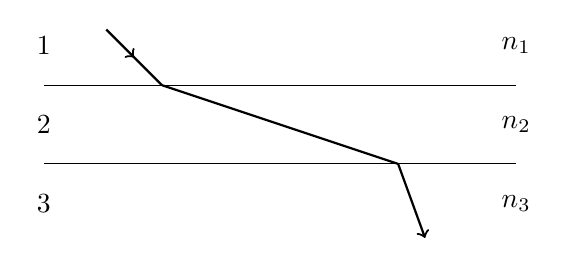
\begin{tikzpicture}
        %% transitions
        \draw (-3,0.5) -- (3,0.5);
        \draw (-3,-0.5) -- (3,-0.5);
        %% Ray
        \draw[thick,->] (-1.5,0.5) -- ++(135:1) -- ++(315:0.5);
        \draw[thick] (-1.5,0.5) -- (1.5,-0.5);
        \draw[thick,->] (+1.5,-0.5) -- ++(290:1);
        %% number labels
        \node[anchor=center] at (-3,1) {1};
        \node[anchor=center] at (-3,0) {2};
        \node[anchor=center] at (-3,-1) {3};
        %% index labels
        \node[anchor=center] at (3,1) {$n_1$};
        \node[anchor=center] at (3,0) {$n_2$};
        \node[anchor=center] at (3,-1) {$n_3$};
    \end{tikzpicture}
    \end{center}
    Which of the following best describes the relation between the indices of refraction?
    \begin{multicols}{2}
    \begin{choices}
        \wrongchoice{$n_1 > n_2 > n_3$}
        \wrongchoice{$n_1 > n_3 > n_2$}
        \wrongchoice{$n_2 > n_1 > n_3$}
        \wrongchoice{$n_2 > n_3 > n_1$}
      \correctchoice{$n_3 > n_1 > n_2$}
    \end{choices}
    \end{multicols}
\end{question}
}


%% PhysicsBowl 1996
%%----------------------------------------
\element{aapt}{ %% Bowl-B2
\begin{question}{bowl-1996-q02}
    A beam of light is directed toward a point $P$ on a boundary as shown to the right.
    \begin{center}
    \begin{tikzpicture}
        %% boundary
        \draw (-3,0) -- (3,0);
        \draw[dashed] (0,-2) -- (0,2);
        \node[anchor=south west] at (-3,0) {$n=1.0$};
        \node[anchor=north west] at (-3,0) {$n=1.5$};
        \fill (0,0) circle (1pt) node[anchor=south west] {$P$};
        %% incoming
        \draw[thick] (135:2) -- (0,0);
        \draw[black,thick,decorate,decoration={markings,mark=at position 0.5 with {\arrow{latex}}}] (135:2) -- (0,0);
        %% refracted
        \foreach \x/\y in {360/A,330/B,315/C,298/D,270/E}
            \draw[thick,->] (0,0) -- (\x:2) node[anchor=center,shift={(\x:1em)},fill=white] {$\y$};
    \end{tikzpicture}
    \end{center}
    Which segment best represents the refracted ray?
    \begin{multicols}{3}
    \begin{choices}[o]
        \wrongchoice{$PA$}
        \wrongchoice{$PB$}
        \wrongchoice{$PC$}
      \correctchoice{$PD$}
        \wrongchoice{$PE$}
    \end{choices}
    \end{multicols}
\end{question}
}

\element{aapt}{ %% Bowl-B2
\begin{question}{bowl-1996-q19}
    Light that has wavelength of \SI{500}{\nano\meter} in air has wavelength \SI{400}{\nano\meter} in a transparent material.
    What is the index of refraction of the material?
    \begin{multicols}{3}
    \begin{choices}
        \wrongchoice{\num{0.64}}
        \wrongchoice{\num{0.80}}
        \wrongchoice{\num{1.00}}
      \correctchoice{\num{1.25}}
        \wrongchoice{\num{1.56}}
    \end{choices}
    \end{multicols}
\end{question}
}

\element{aapt}{ %% Bowl-B2
\begin{question}{bowl-1996-q25}
    Which of the following is \emph{not} possible for the images formed by the lens in the accompanying figure?
    \begin{center}
    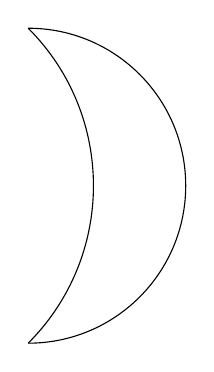
\begin{tikzpicture}
        \draw (0,2) arc (90:-90:2);
        \draw (0,2) arc (45:-45:2.828);
    \end{tikzpicture}
    \end{center}
    \begin{choices}
        \wrongchoice{real and inverted}
        \wrongchoice{real and smaller in size}
        \wrongchoice{real and larger in size}
        \wrongchoice{virtual and erect}
      \correctchoice{virtual and smaller in size}
    \end{choices}
\end{question}
}


%% PhysicsBowl 1995
%%----------------------------------------
\element{aapt}{ %% Bowl-B2
\begin{question}{bowl-1995-q10}
    A plane mirror produces an image that is:
    \begin{choices}
        \wrongchoice{real, inverted, and larger than the object.}
        \wrongchoice{real, upright, and the same size as the object.}
        \wrongchoice{real, upright, and smaller than the object.}
        \wrongchoice{virtual, inverted, and smaller than the object.}
      \correctchoice{virtual, upright, and the same size as the object.}
    \end{choices}
\end{question}
}

\element{aapt}{ %% Bowl-B2
\begin{question}{bowl-1995-q12}
    The principle underlying fiber optics is:
    \begin{choices}
        \wrongchoice{diffraction}
        \wrongchoice{dispersion}
        \wrongchoice{interference}
        \wrongchoice{polarization}
      \correctchoice{total internal reflection}
    \end{choices}
\end{question}
}

\element{aapt}{ %% Bowl-B2
\begin{question}{bowl-1995-q21}
    A diverging lens produces an image of a real object that is:
    \begin{choices}
        \wrongchoice{real, inverted, and larger than the object.}
        \wrongchoice{real, upright, and the same size as the object.}
        \wrongchoice{virtual, inverted, and smaller than the object.}
        \wrongchoice{virtual, upright, and larger than the object.}
      \correctchoice{virtual, upright, and smaller than the object.}
    \end{choices}
\end{question}
}


%% PhysicsBowl 1994
%%----------------------------------------
\element{aapt}{ %% Bowl-B2
\begin{question}{bowl-1994-q11}
    The critical angle of a material is the angle of incidence for which the angle of refraction is:
    \begin{multicols}{3}
    \begin{choices}
        \wrongchoice{\ang{0}}
        \wrongchoice{\ang{30}}
        \wrongchoice{\ang{45}}
      \correctchoice{\ang{90}}
        \wrongchoice{\ang{180}}
    \end{choices}
    \end{multicols}
\end{question}
}

\element{aapt}{ %% Bowl-B2
\begin{question}{bowl-1994-q18}
    An object is located \SI{0.20}{\meter} from a converging lens which
        has a focal length of \SI{0.15}{\meter}.
    Relative to the object, the image formed by the lens will be:
    \begin{choices}
        \wrongchoice{real, erect, and smaller.}
        \wrongchoice{real, inverted, and smaller.}
        \wrongchoice{real, inverted, and larger.}
        \wrongchoice{virtual, erect, and larger.}
        \wrongchoice{virtual, inverted, and smaller.}
    \end{choices}
\end{question}
}


\endinput


